\newpage
\section{Suddivisione del lavoro} \label{SuddivisioneDelLavoro}
	
	La sezione riporta la ripartizione dei ruoli tra i membri del team di sviluppo, basandosi su quanto pianificato.
	
	Vengono seguite le seguenti regole:
	\begin{itemize}
		\item ogni membro deve ricoprire ogni ruolo pianificato almeno una volta
		\item il numero minimo di ore per ruolo che viene ricoperto da un membro in un dato periodo viene fissato a 5 ore
		\item le ore di lavoro svolte da ogni membro per ogni ruolo dovrà essere più o meno equivalente.
     \end{itemize}
     
     Nel preventivo le ore di lavoro impiegate per la formazione personale non vengono rendicontate.
	
	\newpage
	
	\subsection{Dettaglio Fasi}
		\subsubsection{Analisi dei Requisiti}
			La suddivisione dei ruoli tra i vari membri del team di sviluppo nel periodo di Analisi dei Requisiti è la seguente:
			
			\begin{table}[H]
				\begin{detailtable}{\columnwidth}{m{3cm}YYYYYYY}
					\thead{Membro} & 
					\thead{Re} &
					\thead{Am} &
					\thead{An} &
					\thead{Pj} &
					\thead{Pr} &
					\thead{Ve} &
					\thead{Totale}\\\hline\rowcolor{gray!15}
					Ciprian Voinea & 8 & & 9 & & & 7 & 24\\\hline
					Laura Cameran & & 8 & 9 & & & 7 & 24\\\hline\rowcolor{gray!15}
					Matteo Marchiori & 8 & & 9 & & & 7 & 24\\\hline
					Nicola Carlesso & 8 & & 9 & & & 7 & 24\\\hline\rowcolor{gray!15} 
					Samuele Gardin & & 8 & 9 & & & 7 & 24\\\hline 
					Timoty Graziero & & 8 & 9 & & & 7 & 24
				\end{detailtable}
				\caption{Tabella con la suddivisione oraria nel periodo di Analisi dei Rischi}
			\end{table}
			
			\begin{figure}[H]
					\centering
					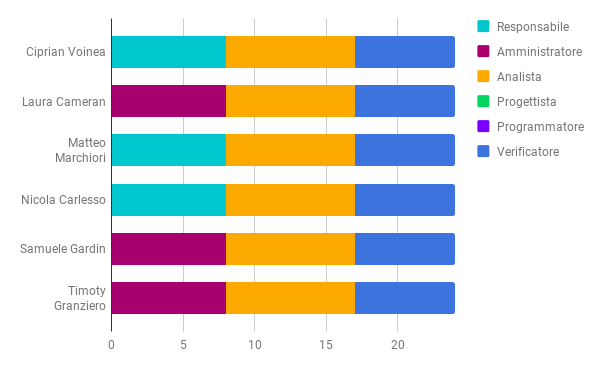
\includegraphics[scale=0.7]{img/Ore_Analisi_dei_Requisiti.png}\\
					\caption{Grafico di suddivisione del lavoro nel periodo di Analisi dei Requisiti}
			\end{figure}
		
		\newpage
		
		\subsubsection{Progettazione della Base Tecnologica}
			La suddivisione dei ruoli tra i vari membri del team di sviluppo nel periodo di Progettazione della Base Tecnologica è la seguente:
			
			\begin{table}[H]
				\begin{detailtable}{\columnwidth}{m{3cm}YYYYYYY}
					\thead{Membro} & 
					\thead{Re} &
					\thead{Am} &
					\thead{An} &
					\thead{Pj} &
					\thead{Pr} &
					\thead{Ve} &
					\thead{Totale}\\\hline\rowcolor{gray!15}
					Ciprian Voinea & & 6 & & 20 & & 14 & 40\\\hline
				    Laura Cameran & 7 & & 7 & 13 & & 23 & 50\\\hline\rowcolor{gray!15}
					Matteo Marchiori & & & & 19 & 23 & 7 & 49\\\hline
					Nicola Carlesso & & 7 & & 20 & 10 & 7 & 44\\\hline\rowcolor{gray!15}
					Samuele Gardin & 8 & & & 13 & 17 & 7 & 45\\\hline
					Timoty Graziero & 7 & 7 & 7 & 15 & & 7 & 43	
				\end{detailtable}
				\caption{Tabella con la suddivisione oraria nel periodo di Progettazione della Base Tecnologica}
			\end{table}
			
			\begin{figure}[H]
					\centering
					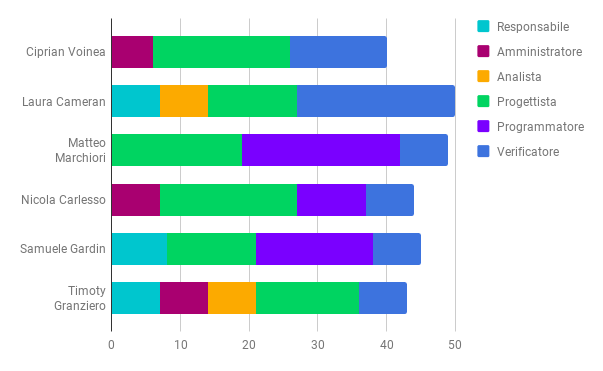
\includegraphics[scale=0.7]{img/Ore_Progettazione_Architetturale.png}\\
					\caption{Grafico di suddivisione del lavoro nel periodo di Progettazione della Base Tecnologica}
			\end{figure}
			
		\newpage
		
		\subsubsection{Progettazione di Dettaglio e Codifica}
			La suddivisione dei ruoli tra i vari membri del team di sviluppo nel periodo di Progettazione di Dettaglio e Codifica è la seguente:
		
			\begin{table}[H]
				\begin{detailtable}{\columnwidth}{m{3cm}YYYYYYY}
					\thead{Membro} & 
					\thead{Re} &
					\thead{Am} &
					\thead{An} &
					\thead{Pj} &
					\thead{Pr} &
					\thead{Ve} &
					\thead{Totale}\\\hline\rowcolor{gray!15}
					Ciprian Voinea & & 6 & & 7 & 20 & 10 & 43\\\hline
					Laura Cameran & 7 & & & 13 & 21 & & 41\\\hline\rowcolor{gray!15}
					Matteo Marchiori & 7 & 6 & & 8 & & 21 & 42\\\hline
					Nicola Carlesso & 8 & & & 7 & 11 & 21 & 47\\\hline\rowcolor{gray!15}
					Samuele Gardin & & 8 & & 16 & & 21 & 45\\\hline
					Timoty Graziero & & & & 14 & 17 & 11 & 42	
				\end{detailtable}
				\caption{Tabella con la suddivisione oraria nel periodo di Progettazione di Dettaglio e Codifica}
			\end{table}
			
			\begin{figure}[H]
					\centering
					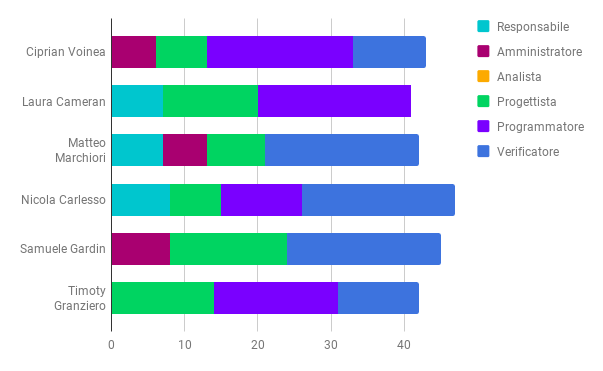
\includegraphics[scale=0.7]{img/Ore_Progettazione_Dettaglio_Codifica.png}\\
					\caption{Grafico di suddivisione del lavoro nel periodo di Progettazione di Dettaglio e Codifica}
			\end{figure}
			
		\newpage
		
		\subsubsection{Validazione e Collaudo}
			La suddivisione dei ruoli tra i vari membri del team di sviluppo nel periodo di Validazione e Collaudo è la seguente:
			
			\begin{table}[H]
				\begin{detailtable}{\columnwidth}{m{3cm}YYYYYYY}
					\thead{Membro} & 
					\thead{Re} &
					\thead{Am} &
					\thead{An} &
					\thead{Pj} &
					\thead{Pr} &
					\thead{Ve} &
					\thead{Totale}\\\hline\rowcolor{gray!15}
					Ciprian Voinea & 8 & & & & & 13 & 21\\\hline
					Laura Cameran & & 5 & & & & 8 & 13\\\hline\rowcolor{gray!15}
					Matteo Marchiori & & 5 & & & & 8 & 13\\\hline
					Nicola Carlesso & & 5 & & & & 8 & 13\\\hline\rowcolor{gray!15}
					Samuele Gardin & 6 & & & & & 8 & 14\\\hline
					Timoty Graziero & 6 & & & & & 13 & 19	
				\end{detailtable}
				\caption{Tabella con la suddivisione oraria nel periodo di Validazione e Collaudo}
			\end{table}
			
			\begin{figure}[H]
					\centering
					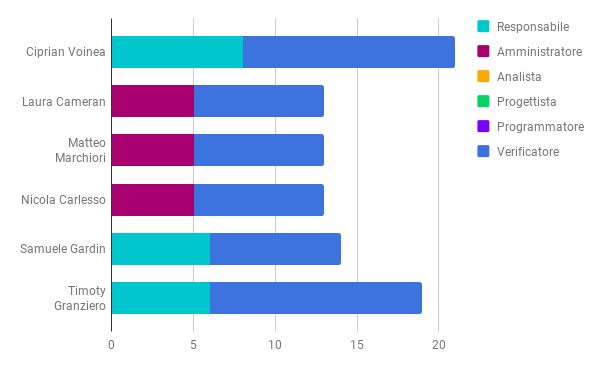
\includegraphics[scale=0.7]{img/Ore_Verifica_Validazione.png}\\
					\caption{Grafico di suddivisione del lavoro nel periodo di Validazione e Collaudo}
			\end{figure}
			
	\newpage

	\subsection{Totali}
		\subsubsection{Ore totali rendicontate}
			Vengono riportate in seguito i totali delle ore rendicontate in preventivo a carico del committente.
			
			\begin{table}[H]
				\begin{detailtable}{\columnwidth}{m{3cm}YYYYYYY}
					\thead{Membro} & 
					\thead{Re} &
					\thead{Am} &
					\thead{An} &
					\thead{Pj} &
					\thead{Pr} &
					\thead{Ve} &
					\thead{Totale}\\\hline\rowcolor{gray!15}
					Ciprian Voinea & 8 & 12 & & 27 & 20 & 37 & 104\\\hline
					Laura Cameran & 14 & 5 & 7 & 26 & 21 & 31 & 104\\\hline\rowcolor{gray!15}
					Matteo Marchiori & 7 & 11 & & 27 & 23 & 36 & 104\\\hline
					Nicola Carlesso & 8 & 12 & & 27 & 21 & 36 & 104\\\hline\rowcolor{gray!15}
					Samuele Gardin & 14 & 8 & & 29 & 17 & 36 & 104\\\hline
					Timoty Graziero & 13 & 7 & 7 & 29 & 17 & 31 & 104	
				\end{detailtable}
				\caption{Tabella con i totali delle ore rendicontate}
			\end{table}
			
			\begin{figure}[H]
					\centering
					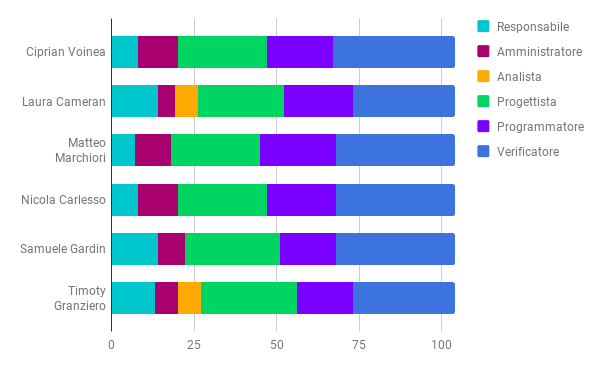
\includegraphics[scale=0.7]{img/Ore_Rendicontate.png}\\
					\caption{Grafico di confronto con le ore rendicontate}
			\end{figure}
		
		\newpage
	
		\subsubsection{Ore totali con investimento}
			Vengono riportate in seguito i totali delle ore rendicontate in preventivo a carico del committente e delle ore di investimento.
			
			\begin{table}[H]
				\begin{detailtable}{\columnwidth}{m{3cm}YYYYYYY}
					\thead{Membro} & 
					\thead{Re} &
					\thead{Am} &
					\thead{An} &
					\thead{Pj} &
					\thead{Pr} &
					\thead{Ve} &
					\thead{Totale}\\\hline\rowcolor{gray!15}
					Ciprian Voinea & 20 & 14 & 11 & 31 & 22 & 46 & 144\\\hline
					Laura Cameran & 18 & 15 & 11 & 30 & 23 & 40 & 144\\\hline\rowcolor{gray!15}
					Matteo Marchiori & 19 & 13 & 11 & 31 & 25 & 45 & 144\\\hline
					Nicola Carlesso & 20 & 14 & 11 & 31 & 23 & 45 & 144\\\hline\rowcolor{gray!15}
					Samuele Gardin & 18 & 18 & 11 & 33 & 19 & 45 & 144\\\hline
					Timoty Graziero & 17 & 17 & 18 & 33 & 19 & 40 & 144	
				\end{detailtable}
				\caption{Tabella con i totali delle ore rendicontate e di investimento}
			\end{table}
			
			\begin{figure}[H]
					\centering
					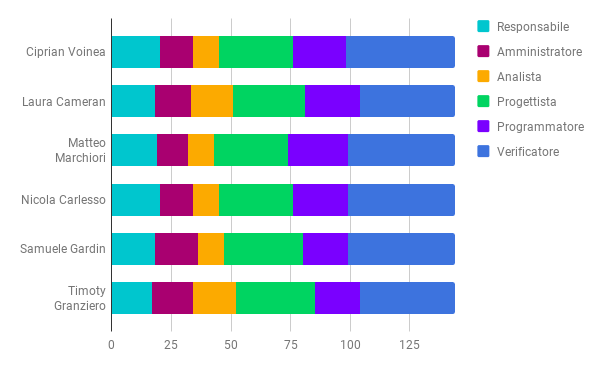
\includegraphics[scale=0.7]{img/Ore_Totali.png}\\
					\caption{Grafico di confronto con le ore totali}
			\end{figure}